\documentclass[a4paper, 12pt]{article}

% Includes 
\usepackage[utf8]{inputenc} % UTF-8 encode 
\usepackage[english, russian]{babel}
\usepackage{geometry} % adjust page layout 
\usepackage{graphicx} 
\usepackage{hyperref} 
\usepackage{amsmath} % math formulas 
\usepackage{setspace} % for set line spacing 
\usepackage{indentfirst} % indent on a first line after the paragraph 
% \usepackage{pgfplots} % for plots 
\usepackage{listings} % for code listings 
\usepackage{xcolor} % colors (used for listings)
\usepackage{sourcecodepro} % for another monospaced font 

% debug
% \usepackage{showframe} % frame borders for demonstration 


%%% Custom commands
% commands for unnumbered sections
\newcommand{\usection}[1]{\section*{#1} \addcontentsline{toc}{section}{\protect\numberline{}#1}}
\newcommand{\usubsection}[1]{\subsection*{#1} \addcontentsline{toc}{subsection}{\protect\numberline{}#1}}
\newcommand{\usubsubsection}[1]{\subsubsection*{#1} \addcontentsline{toc}{subsubsection}{\protect\numberline{}#1}}


% Redefinition of section and subsection numbering style
\def\thesection{\arabic{section}.}
\def\thesubsection{\arabic{section}.\arabic{subsection}.}
\def\thesubsubsection{\arabic{section}.\arabic{subsection}.\arabic{subsubsection}.}


% Settings for links 
\hypersetup{
    colorlinks,
    citecolor=black,
    filecolor=black,
    linkcolor=black,
    urlcolor=blue
}


% Layout
\geometry{
	left=17mm,
	top=17mm,
	right=17mm,
	bottom=20mm,
	marginparsep=0mm,
	marginparwidth=0mm,
	headheight=8mm,
	headsep=5mm, 
}

\linespread{1.5} % line spacing
\setlength{\parskip}{\baselineskip}  % Add space between paragraphs
\renewcommand*{\arraystretch}{0.8} % Space between table rows

% overfull hbox settings
\tolerance 5000 % default 200, max 10000
\hbadness 10000 % default 1000, max 10000
\emergencystretch 10pt  % default 0pt, how much the lines can stretch for the sake of good line breaks
\hfuzz 10pt % ignore overfull box less than 
\widowpenalty=5000 % no lines at the start of the page
\vfuzz \hfuzz % don't care about underfull vbox if overfull is acceptable
\raggedbottom % if the page is not filled, align the content to the bottom


% Redefinition of table of contents command to get centered heading
\makeatletter
\renewcommand\tableofcontents{ 
  \begin{singlespace}
    \null\hfill\textbf{\Large\contentsname}\hfill\null\par
    \@mkboth{\MakeUppercase\contentsname}{\MakeUppercase\contentsname}%
    \@starttoc{toc}
  \end{singlespace}
}
\makeatother


% Listings settings
\definecolor{codegreen}{rgb}{0, 0.6, 0}
\definecolor{codegray}{rgb}{0.5, 0.5, 0.5}
\definecolor{codepurple}{rgb}{0.58, 0, 0.82}
\definecolor{backcolour_gray}{rgb}{0.98, 0.98, 0.98}

\lstdefinestyle{cpp_white}{
  language=C++,
  backgroundcolor=\color{backcolour_gray},   
  commentstyle=\color{codegreen},
  keywordstyle=\color{blue},
  numberstyle=\tiny\color{codegray},
  stringstyle=\color{codepurple},
  basicstyle=\ttfamily\small\singlespacing,
  breakatwhitespace=true,         
  breaklines=true,                 
  captionpos=b, % t/b                  
  keepspaces=true,                 
  numbers=none, % none/left/rigth                    
  numbersep=5pt,                  
  showspaces=false,                
  showstringspaces=false,
  showtabs=false,                  
  tabsize=2,
  frame=single, % none/leftline/topline/bottomline/lines/single/shadowbox
  rulecolor=\color{gray}, % frame color 
}


\lstset{style=cpp_white}
% \lstset { %
%     language=C++,
%     backgroundcolor=\color{black!5}, % set backgroundcolor
%     basicstyle=\footnotesize,% basic font setting
% }


% For title page
\def\name{Отчет по лабораторной работе №2} 
\def\subname{Геометрические преобразования изображений}
\def\madeby{Новичков Дмитрий, ТЕХ.ЗРЕНИЕ 1.1}
\def\teacher{Шаветов С. В.}
\begin{document}

% Title page 
\begin{titlepage}

\thispagestyle{empty}

\title{


\includegraphics[width=4cm]{media/ITMO_logo.png} 

\vspace{1em}
\begin{center}
\large\textsc{\textbf{Национальный исследовательский университет ИТМО}}
\vspace{1em}
\end{center}
% \vspace{4em}

\begin{center}
\large\textsc{\textbf{Дисциплина: Техническое зрение}}
\vspace{1em}
\end{center}

\begin{center}
\large\textsc{\textbf{\name}}

\vspace{1em}
``\subname'' 

\end{center}

\vspace{3em}

\begin{flushright}
\normalsize{ 
Выполнили: \\ \textbf{\madeby} 

Преподаватель: \\ \textbf{\teacher} 
}
\end{flushright}	

\vfill

% \vspace{4em}

\begin{center}
\small{Санкт-Петербург, \the\year}
\end{center}
}


\author{}
\date{}
\maketitle
\thispagestyle{empty}
\end{titlepage} % Title page

\tableofcontents % Table of contents
\pagebreak

\href{https://github.com/mfclabber/itmo-cv-labs/tree/main/lab5}{Исходный код на GitHub}. 

Для удобства отладки и сборки используется средство автоматизации сборки ПО CMake:
\begin{lstlisting}[style=cpp_white, caption={CMakeLists.txt для сборки проекта}]
cmake_minimum_required(VERSION 2.8)

project( CV_LW4 )
find_package( OpenCV REQUIRED )

include_directories( ${OpenCV_INCLUDE_DIRS} )
add_executable( ${PROJECT_NAME}  src/lab2.cpp )

target_link_libraries( ${PROJECT_NAME} ${OpenCV_LIBS} )
\end{lstlisting}

\section{Поиск прямых}

Для удобства работы и модульности Л/Р были созданы следующие функции и структура:

\begin{enumerate}
\item Структура func, которая предназначена для инкапсуляции результатов преобразования Хафа различными способами.
Также данная структура помогает избежать использования boost::any для получения различных типов данных из функций, которые будут описаны ниже. 
Главный недостаток boost::any заключается в потери "типов" при преобразовании.
\item Функции "canny hough tranform" и "ordinary hough tranform" применяют преобразования Хафа к изображению, полученному после применения оператора Кэнни и обычной бинаризации соответственно.
\item Статическая функция func::comp используется как компаратор для сравнения длин найденных линий в функциях std::max element и std::min element.
\item Статическая функкция func::length line возвращает длину линии.
\end{enumerate}

\begin{lstlisting}[style=cpp_white, caption={Вспомогательные функции и структура}]
struct func{
    func(std::vector<cv::Vec4i>& lines, cv::Mat& image): lines{lines}, image{image} {};
    std::vector<cv::Vec4i> lines;
    cv::Mat image;
    static bool comp(cv::Vec4i& , cv::Vec4i&);
    static uint lenght_line(cv::Vec4i&);
};


func canny_hough_tranform(cv::Mat& image){

    cv::Mat image_new, image_out = image.clone();
    cv::Canny(image, image_new, 50, 200);
    std::vector<cv::Vec4i> linesP;

    HoughLinesP(image_new, linesP, 1, CV_PI / 150, 80, 40, 4);

    for (int i = 0; i < linesP.size(); ++i){
        cv::Vec4i I = linesP[i];
        cv::line(image_out, cv::Point(I[0], I[1]),
                            cv::Point(I[2], I[3]),
                            cv::Scalar(0, 255, 0), 
                                    1, cv::LINE_AA);

        cv::circle(image_out, cv::Point(I[0], I[1]), 1,
                                        (127, 0, 60), 5, 
                                            cv::LINE_AA);

        cv::circle(image_out, cv::Point(I[2], I[3]), 1, 
                                        (0, 0, 255), 5, 
                                            cv::LINE_AA);
    }

    return func(linesP, image_out);
}



func ordinary_hough_tranform(cv::Mat& image){

    cv::Mat image_new, image_out = image.clone();
    cv::cvtColor(image, image_new, cv::COLOR_BGR2GRAY);

    cv::threshold(image_new, image_new, 50, 255, cv::THRESH_BINARY);

    std::vector<cv::Vec4i> linesP;

    HoughLinesP(image_new, linesP, 1, CV_PI / 180, 50, 50, 15);

    for (int i = 0; i < linesP.size(); ++i){
        cv::Vec4i I = linesP[i];
        cv::line(image_out, cv::Point(I[0], I[1]),
                            cv::Point(I[2], I[3]),
                            cv::Scalar(0, 255, 0), 
                                    1, cv::LINE_AA);

        cv::circle(image_out, cv::Point(I[0], I[1]), 1,
                                        (127, 0, 60), 5, 
                                            cv::LINE_AA);

        cv::circle(image_out, cv::Point(I[2], I[3]), 1, 
                                        (0, 0, 255), 5, 
                                            cv::LINE_AA);
    }
    
    return func(linesP, image_out);
}

bool func::comp(cv::Vec4i& l1, cv::Vec4i& l2){
    return (std::sqrt(std::pow(abs(l1[2] - l1[0]), 2) + std::pow(abs(l1[3] - l1[1]), 2)) < 
            std::sqrt(std::pow(abs(l2[2] - l2[0]), 2) + std::pow(abs(l2[3] - l2[1]), 2)));
}

uint func::lenght_line(cv::Vec4i& l){
    return std::sqrt(std::pow(abs(l[2] - l[0]), 2) + 
                        std::pow(abs(l[3] - l[1]), 2));
}
\end{lstlisting}

\begin{lstlisting}[style=cpp_white, caption={Общий код для поиска прямых с помощью преобразования Хафа}]
// GRAYSCALE

cv::Mat image;
image = cv::imread(path + "/source/test.png", 1);

func output = ordinary_hough_tranform(image);

std::cout << "MAX LENGTH = " << func::lenght_line(*std::max_element(output.lines.begin(), output.lines.end(), func::comp)) <<
                "\nMIN LENGTH = " << func::lenght_line(*std::min_element(output.lines.begin(), output.lines.end(), func::comp)) <<
                "\nNUMBER OF LINES = " << output.lines.size();


cv::imwrite(path + "/outputs/image1_ordinary.png", output.image);
cv::imshow("image", output.image);
cv::waitKey();



// CANNY

cv::Mat image;
image = cv::imread(path + "/source/test.png", 1);

func output = canny_hough_tranform(image);

std::cout << "MAX LENGTH = " << func::lenght_line(*std::max_element(output.lines.begin(), output.lines.end(), func::comp)) <<
                "\nMIN LENGTH = " << func::lenght_line(*std::min_element(output.lines.begin(), output.lines.end(), func::comp)) <<
                "\nNUMBER OF LINES = " << output.lines.size();


cv::imwrite(path + "/outputs/image1_canny.png", output.image);
cv::imshow("image", output.image);
cv::waitKey();
\end{lstlisting}

Синие точки означают конец линии, черные - начало.

\subsection{Изображение №1}

\begin{figure}[H]
    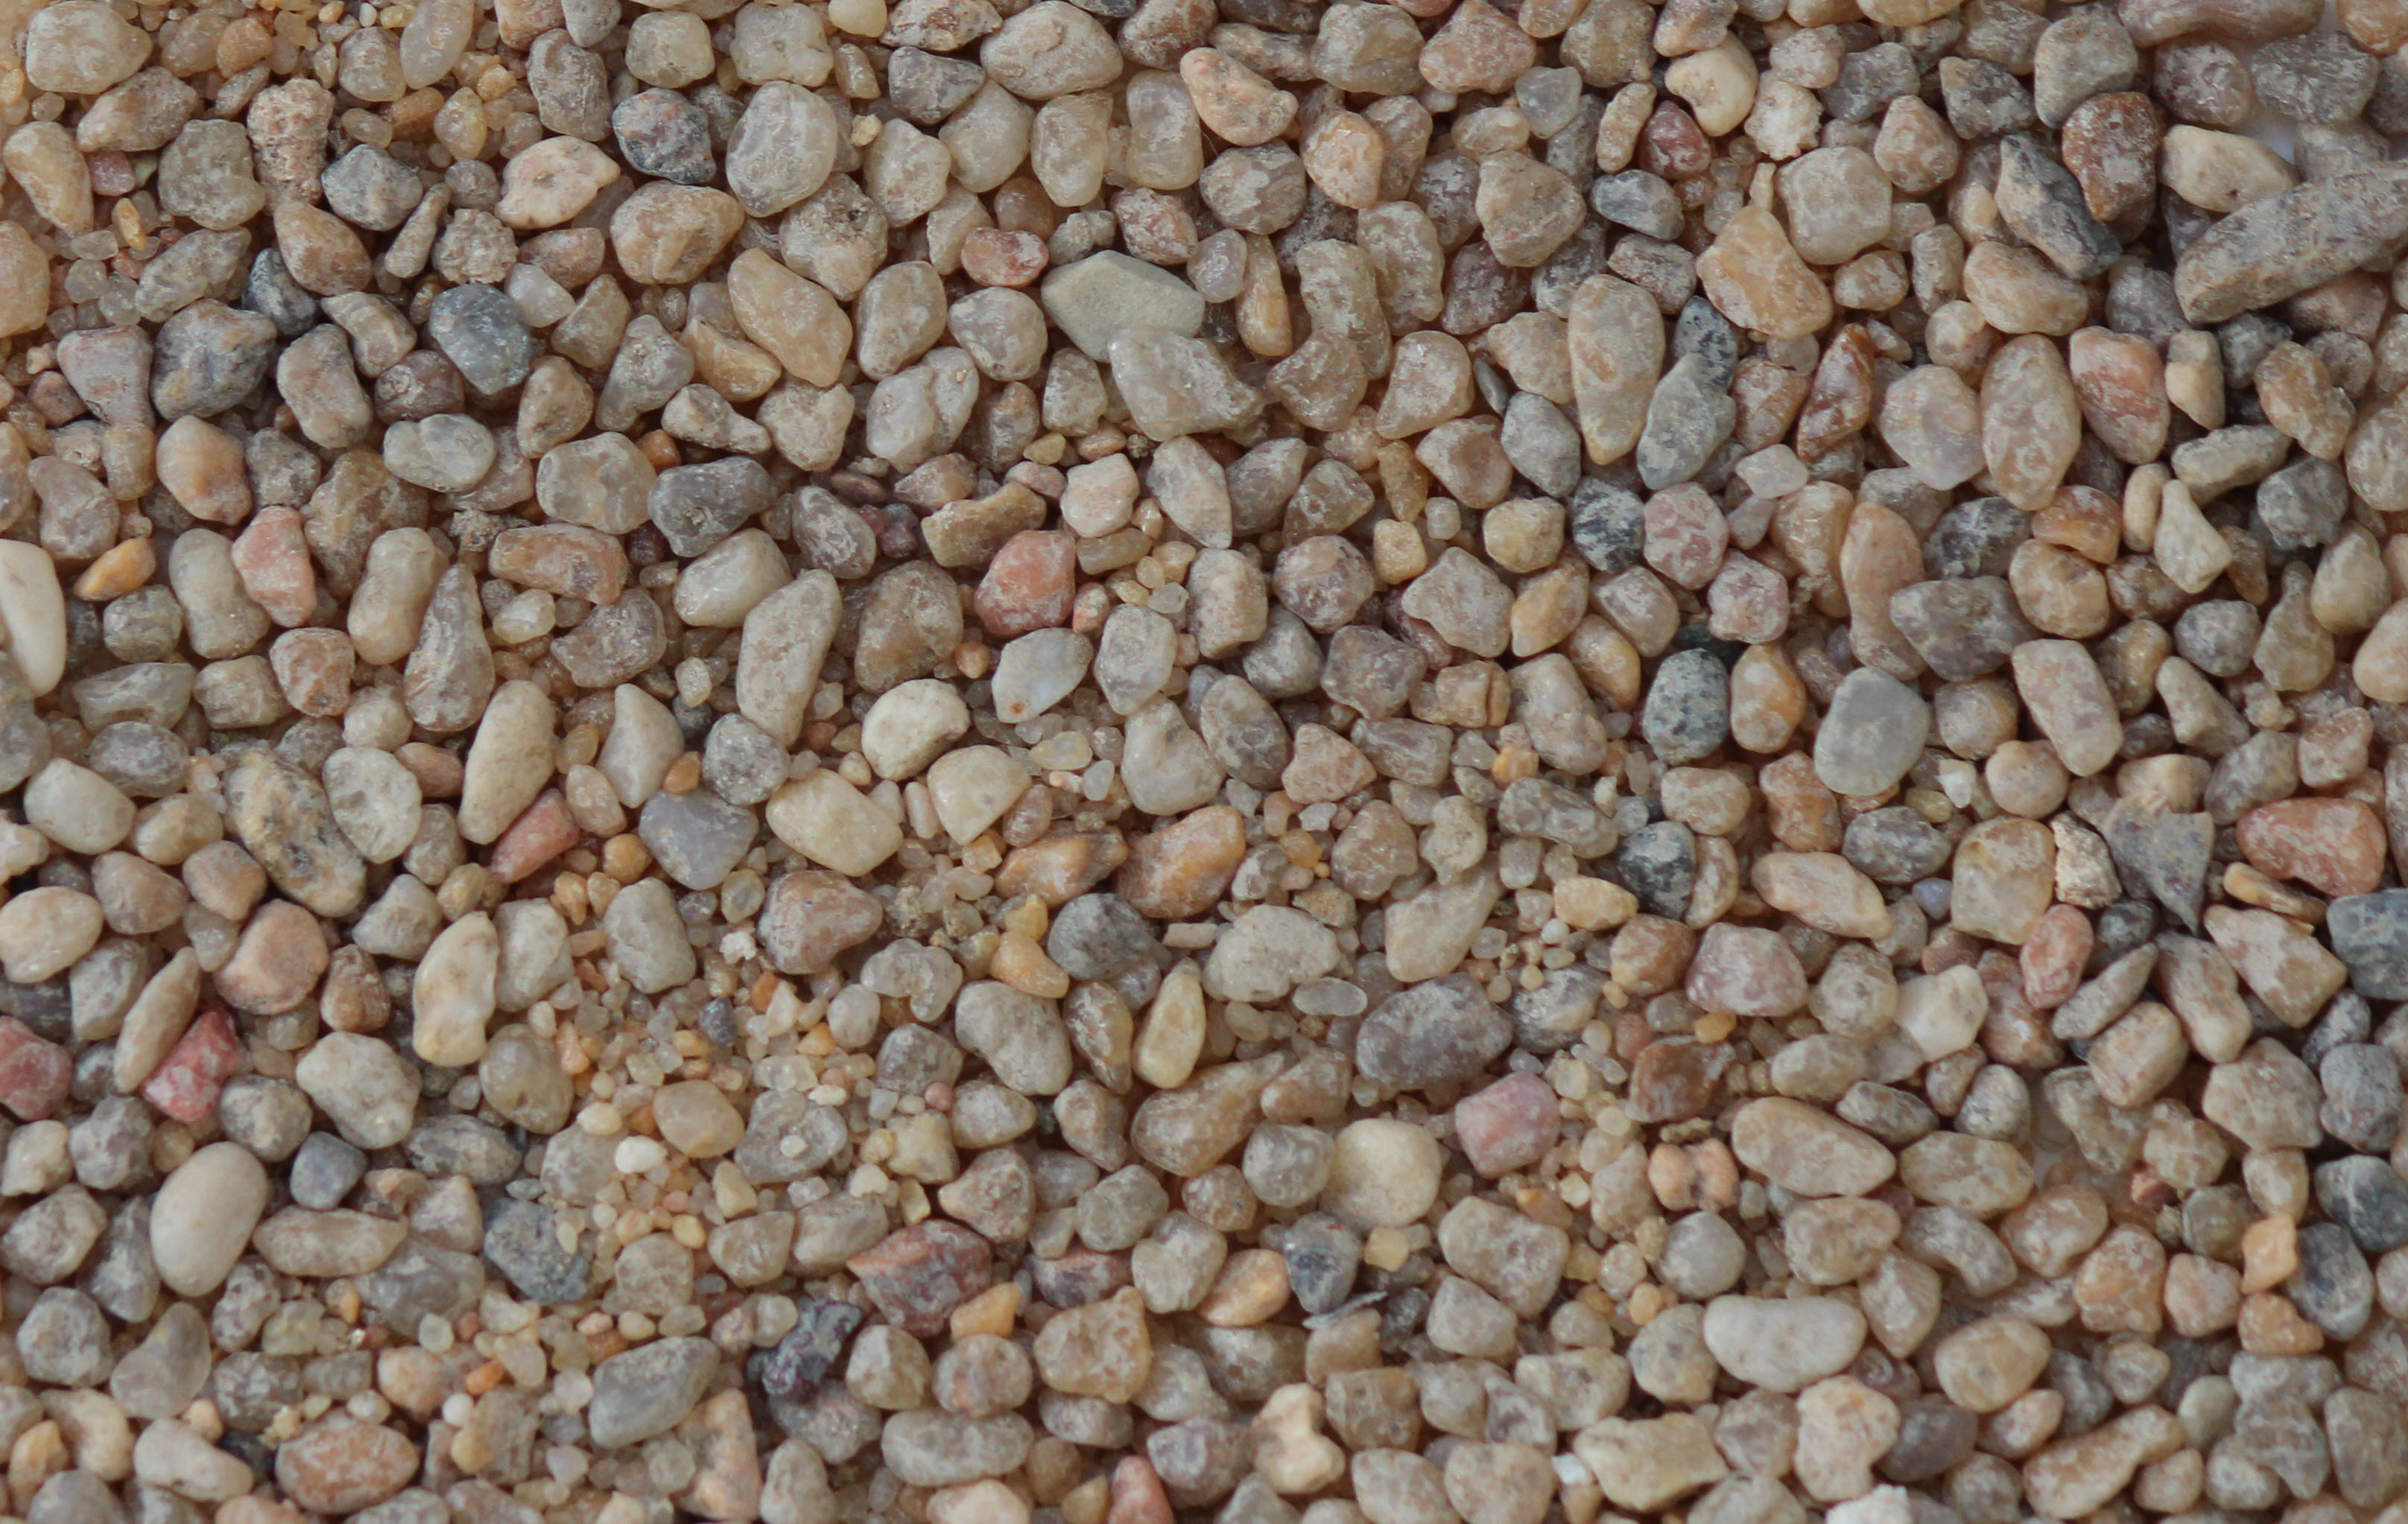
\includegraphics[width=\textwidth]{../source/test.png}
    \caption{Исходное изображение}
    \label{fig:source_image}
\end{figure}

\subsubsection{Исходное изображение}

\begin{figure}[H]
    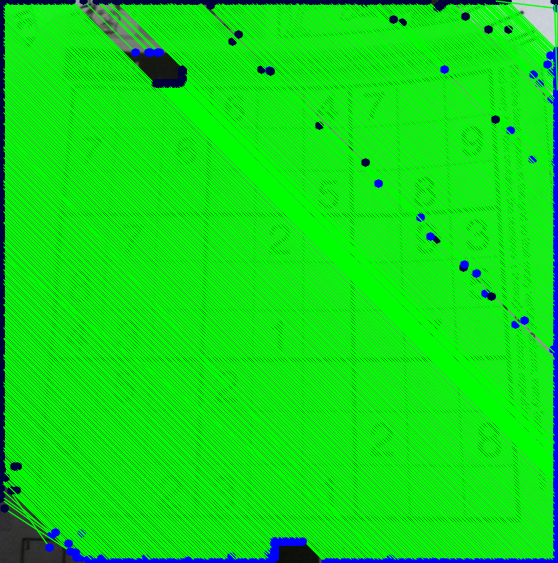
\includegraphics[width=\textwidth]{../outputs/image1_ordinary.png}
    \caption{Результат преобразования Хафа}
    \label{fig:image1_ordinary}
\end{figure}
\ \\
MAX LENGTH = 1279 \\
MIN LENGTH = 50 \ \\
NUMBER OF LINES = 2946

Данное хаотичное поведение объясняется тем, что на вход преобразованию поступило простое бинаризированное по порогу изображение,
 на котором отсутствуют четкие границы (из-за ручного подбора порога), следовательно присутствует много точек, через которые можно провести линии. 

\subsubsection{Обработанное алгоритмом Кэнни}

\begin{figure}[H]
    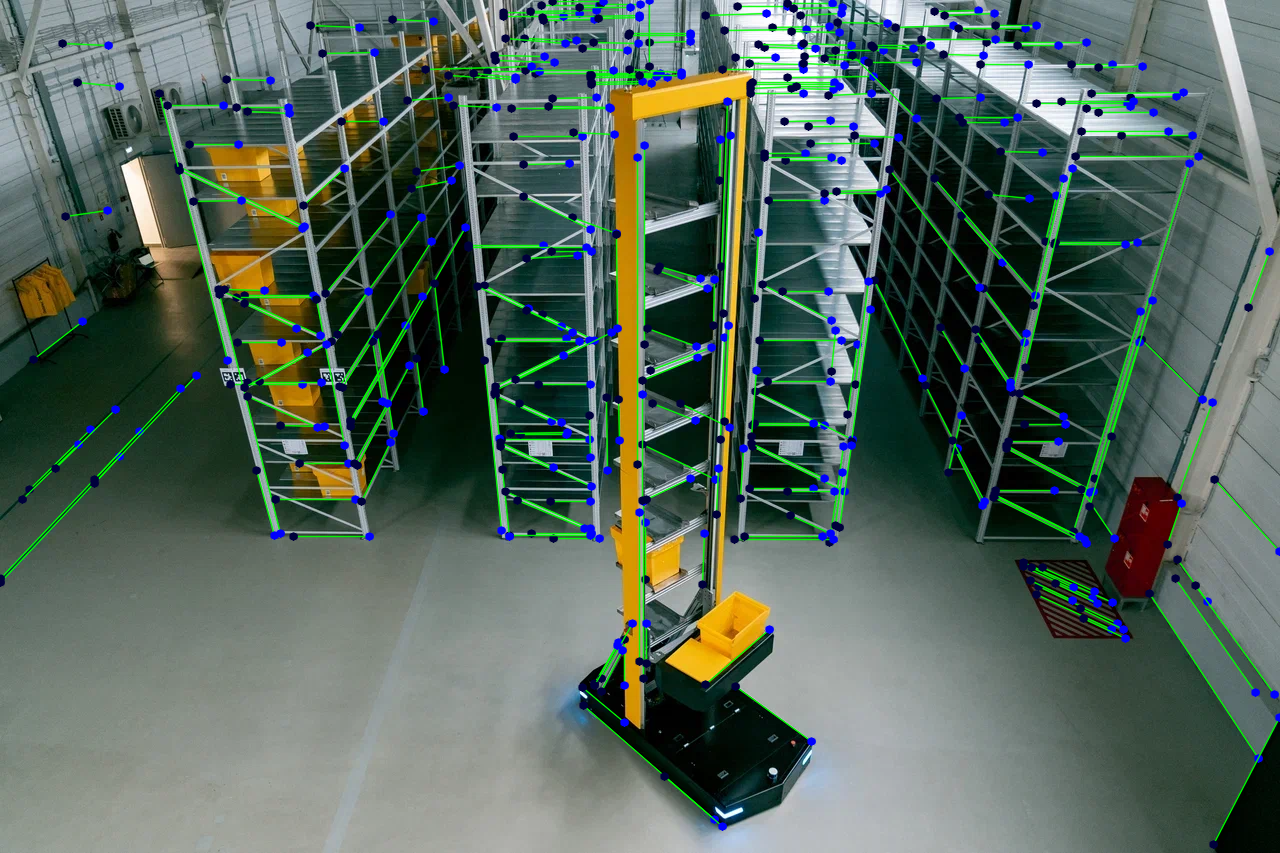
\includegraphics[width=\textwidth]{../outputs/image1_canny.png}
    \caption{Результат преобразования Хафа}
    \label{fig:image1_canny}
\end{figure}
\ \\
MAX LENGTH = 329 \\
MIN LENGTH = 40 \ \\
NUMBER OF LINES = 314


\subsection{Изображение №2}

\begin{figure}[H]
    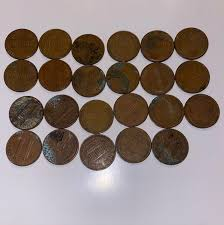
\includegraphics[width=\textwidth]{../source/2.png}
    \caption{Исходное изображение}
    \label{fig:source_image}
\end{figure}

\subsubsection{Исходное изображение}

\begin{figure}[H]
    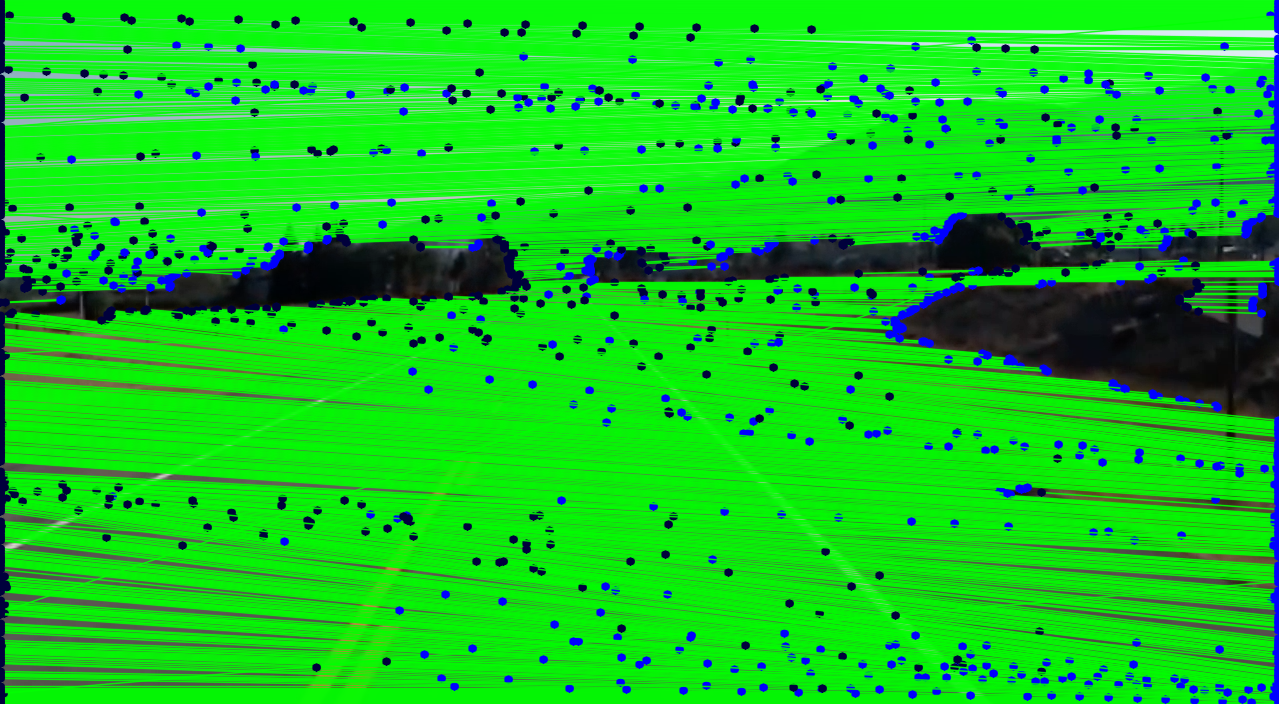
\includegraphics[width=\textwidth]{../outputs/image2_ordinary.png}
    \caption{Результат преобразования Хафа}
    \label{fig:image2_ordinary}
\end{figure}
\ \\
MAX LENGTH = 1290 \\
MIN LENGTH = 50 \ \\
NUMBER OF LINES = 984

\subsubsection{Обработанное алгоритмом Кэнни}

\begin{figure}[H]
    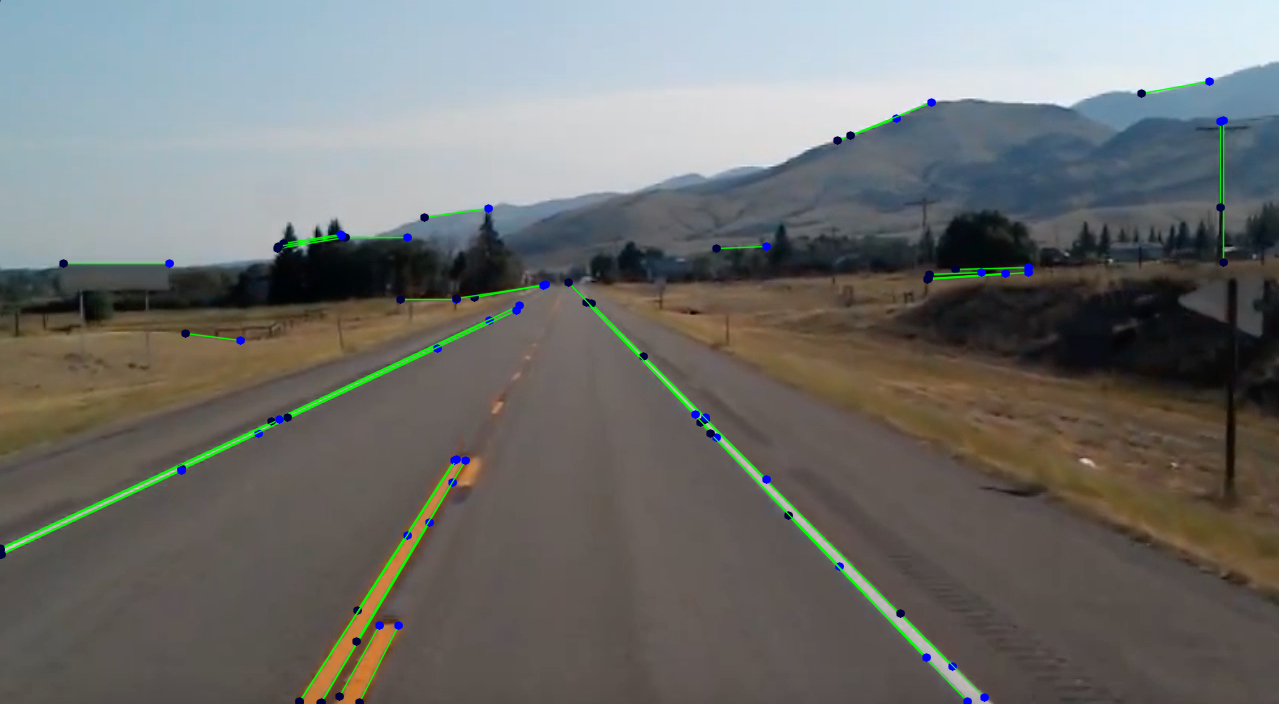
\includegraphics[width=\textwidth]{../outputs/image2_canny.png}
    \caption{Результат преобразования Хафа}
    \label{fig:image2_canny}
\end{figure}
\ \\
MAX LENGTH = 5339 \\
MIN LENGTH = 50 \ \\
NUMBER OF LINES = 44


\subsection{Изображение №3}

\begin{figure}[H]
    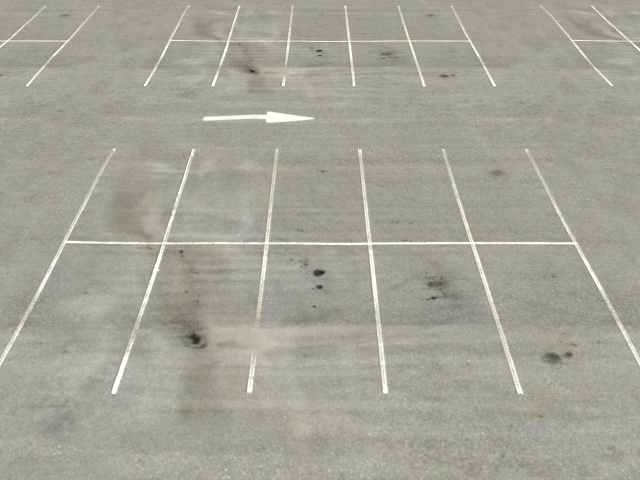
\includegraphics[width=\textwidth]{../source/4.png}
    \caption{Исходное изображение}
    \label{fig:source_image}
\end{figure}

\subsubsection{Исходное изображение}

\begin{figure}[H]
    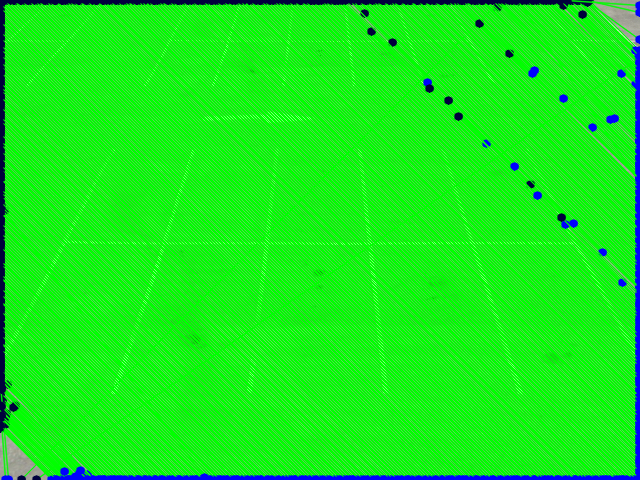
\includegraphics[width=\textwidth]{../outputs/image3_ordinary.png}
    \caption{Результат преобразования Хафа}
    \label{fig:image3_ordinary}
\end{figure}
\ \\
MAX LENGTH = 735 \\
MIN LENGTH = 53 \ \\
NUMBER OF LINES = 738

\subsubsection{Обработанное алгоритмом Кэнни}

\begin{figure}[H]
    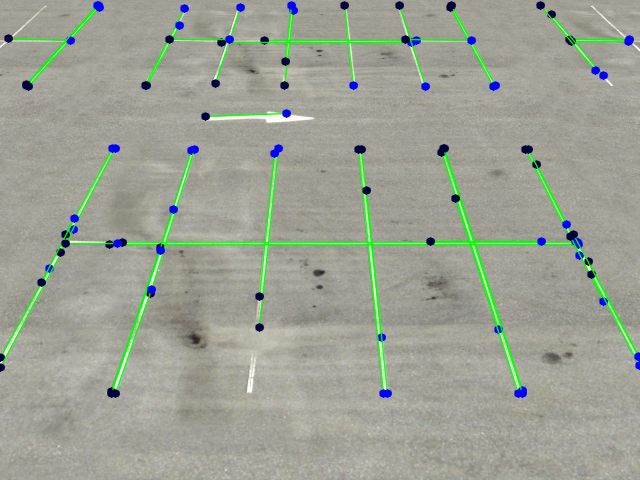
\includegraphics[width=\textwidth]{../outputs/image3_canny.png}
    \caption{Результат преобразования Хафа}
    \label{fig:image3_canny}
\end{figure}
\ \\
MAX LENGTH = 469 \\
MIN LENGTH = 52 \ \\
NUMBER OF LINES = 52

\section{Поиск окружностей}

\begin{lstlisting}[style=cpp_white, caption={Общий код для поиска окружностей с помощью преобразования Хафа}]
cv::Mat image, gray;
cv::cvtColor(image, gray, cv::COLOR_BGR2GRAY);
cv::medianBlur(gray, gray, 5);

std::vector<cv::Vec3f> circles;

cv::HoughCircles(gray, circles, cv::HOUGH_GRADIENT, 1,
gray.rows/16, // change this value to detect circles with different distances to each other
100, 30, 50, 55 // change the last two parameters
// (min_radius & max_radius) to detect larger circles
);
for( size_t i = 0; i < circles.size(); i++ )
{
    cv::Vec3i c = circles[i];
    cv::Point center = cv::Point(c[0], c[1]);
    // circle center
    cv::circle(image, center, 1, cv::Scalar(255,0,0), 3, cv::LINE_AA);
    // circle outline
    int radius = c[2];
    cv::circle(image, center, radius, cv::Scalar(255,0,0), 3, cv::LINE_AA);
}
cv::imwrite(path + "/outputs/image6_ordinary_r50.png", image);
cv::imshow("detected circles", image);
cv::waitKey();


cv::HoughCircles(gray, circles, cv::HOUGH_GRADIENT, 1,
gray.rows/16, // change this value to detect circles with different distances to each other
100, 30, 50, 65 // change the last two parameters
// (min_radius & max_radius) to detect larger circles
);
for( size_t i = 0; i < circles.size(); i++ )
{
    cv::Vec3i c = circles[i];
    cv::Point center = cv::Point(c[0], c[1]);
    // circle center
    cv::circle(image, center, 1, cv::Scalar(255,0,0), 3, cv::LINE_AA);
    // circle outline
    int radius = c[2];
    cv::circle(image, center, radius, cv::Scalar(255,0,0), 3, cv::LINE_AA);
}
cv::imwrite(path + "/outputs/image6_ordinary_r5065.png", image);
cv::imshow("detected circles", image);
cv::waitKey();


// CANNY

cv::cvtColor(image, gray, cv::COLOR_BGR2GRAY);
cv::Canny(gray, gray, 50, 200);

std::vector<cv::Vec3f> circles;

cv::HoughCircles(gray, circles, cv::HOUGH_GRADIENT, 1,
gray.rows/16, // change this value to detect circles with different distances to each other
100, 30, 50, 55 // change the last two parameters
// (min_radius & max_radius) to detect larger circles
);
for( size_t i = 0; i < circles.size(); i++ )
{
    cv::Vec3i c = circles[i];
    cv::Point center = cv::Point(c[0], c[1]);
    // circle center
    cv::circle(image, center, 1, cv::Scalar(255,0,0), 3, cv::LINE_AA);
    // circle outline
    int radius = c[2];
    cv::circle(image, center, radius, cv::Scalar(255,0,0), 3, cv::LINE_AA);
}
cv::imwrite(path + "/outputs/image6_canny_r50.png", image);
cv::imshow("detected circles", image);
cv::waitKey();


cv::HoughCircles(gray, circles, cv::HOUGH_GRADIENT, 1,
gray.rows/16, // change this value to detect circles with different distances to each other
100, 30, 50, 65 // change the last two parameters
// (min_radius & max_radius) to detect larger circles
);
for( size_t i = 0; i < circles.size(); i++ )
{
    cv::Vec3i c = circles[i];
    cv::Point center = cv::Point(c[0], c[1]);
    // circle center
    cv::circle(image, center, 1, cv::Scalar(255,0,0), 3, cv::LINE_AA);
    // circle outline
    int radius = c[2];
    cv::circle(image, center, radius, cv::Scalar(255,0,0), 3, cv::LINE_AA);
}
cv::imwrite(path + "/outputs/image6_canny_r5065.png", image);
cv::imshow("detected circles", image);
cv::waitKey();// image = cv::imread(path + "/source/6.png", 1);
\end{lstlisting}

\subsection{Изображение №1}

\begin{figure}[H]
    \centering
    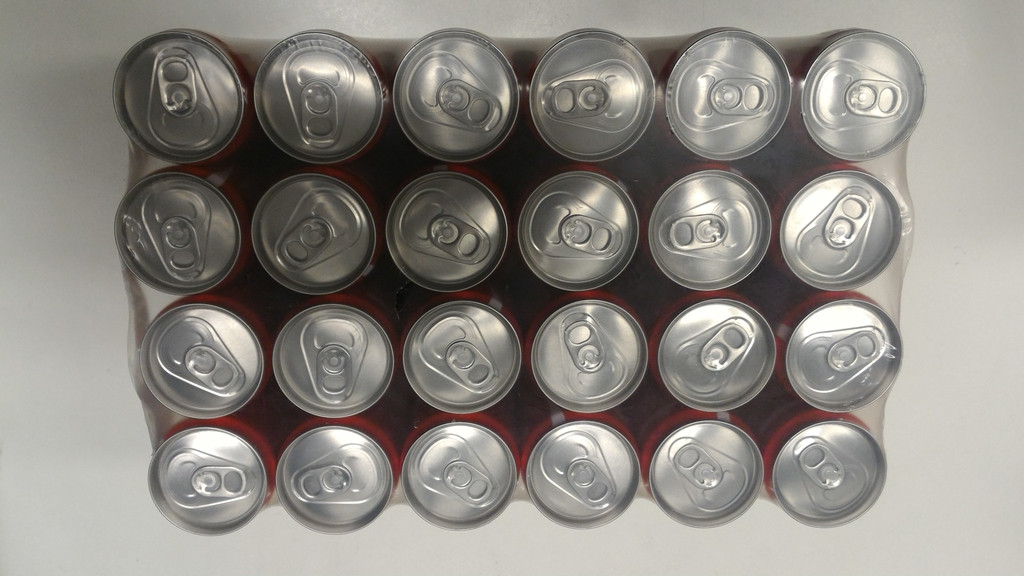
\includegraphics[width=0.9\textwidth]{../source/6.png}
    \caption{Исходное изображение}
    \label{fig:image_source}
\end{figure}

\subsubsection{Исходное изображение}

% \paragraph{Поиск окружностей определенного радиуса}

\begin{figure}[H]
    \centering
    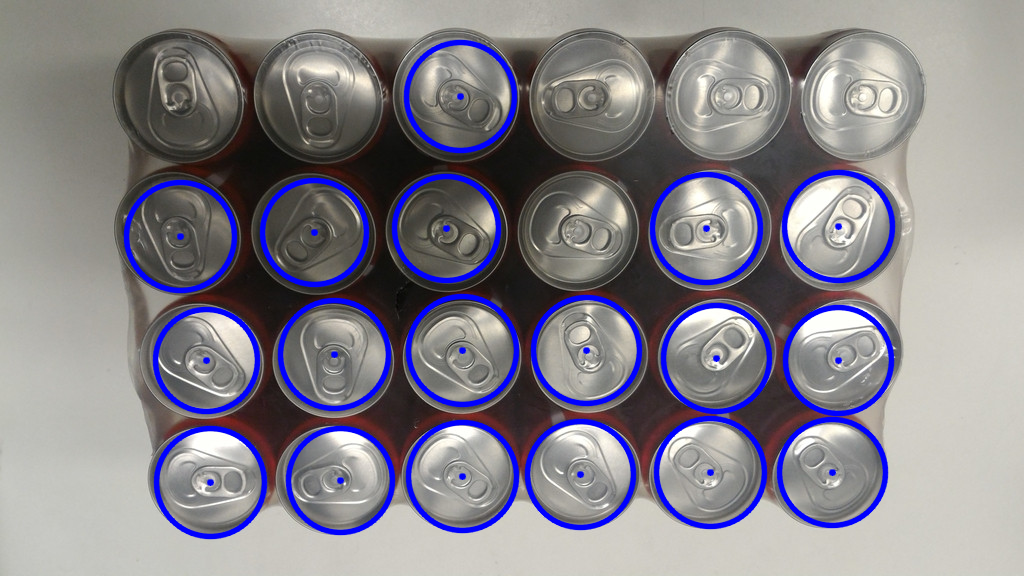
\includegraphics[width=0.9\textwidth]{../outputs/image6_ordinary_r50.png}
    \caption{Результат преобразования Хафа для окружностей радиуса 50}
\end{figure}

% \paragraph{Поиск окружностей определенного диапазона радиусов}

\begin{figure}[H]
    \centering
    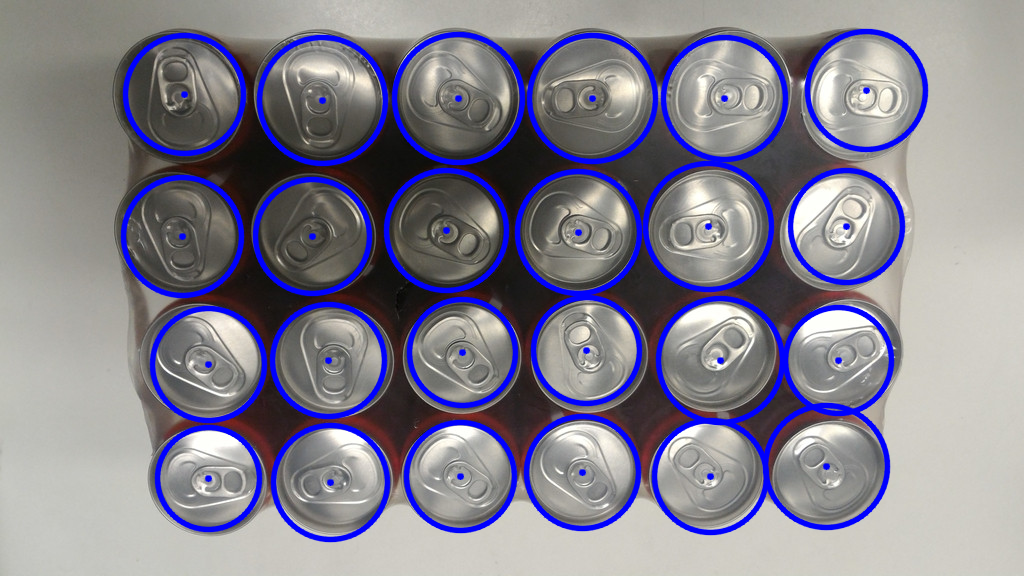
\includegraphics[width=0.9\textwidth]{../outputs/image6_ordinary_r5065.png}
    \caption{Результат преобразования Хафа для окружностей диапазона радиусов $[50, 65]$}
\end{figure}

\subsubsection{Обработанное алгоритмом Кэнни}

% \paragraph{Поиск окружностей определенного радиуса}

\begin{figure}[H]
    \centering
    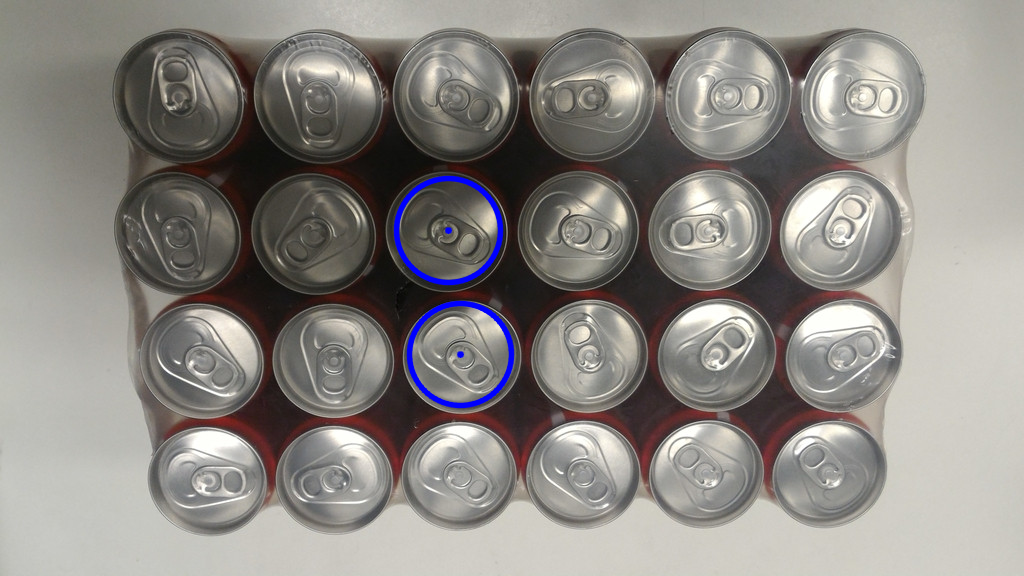
\includegraphics[width=0.9\textwidth]{../outputs/image6_canny_r50.png}
    \caption{Результат преобразования Хафа для окружностей радиуса 50}
\end{figure}

% \paragraph{Поиск окружностей определенного диапазона радиусов}

\begin{figure}[H]
    \centering
    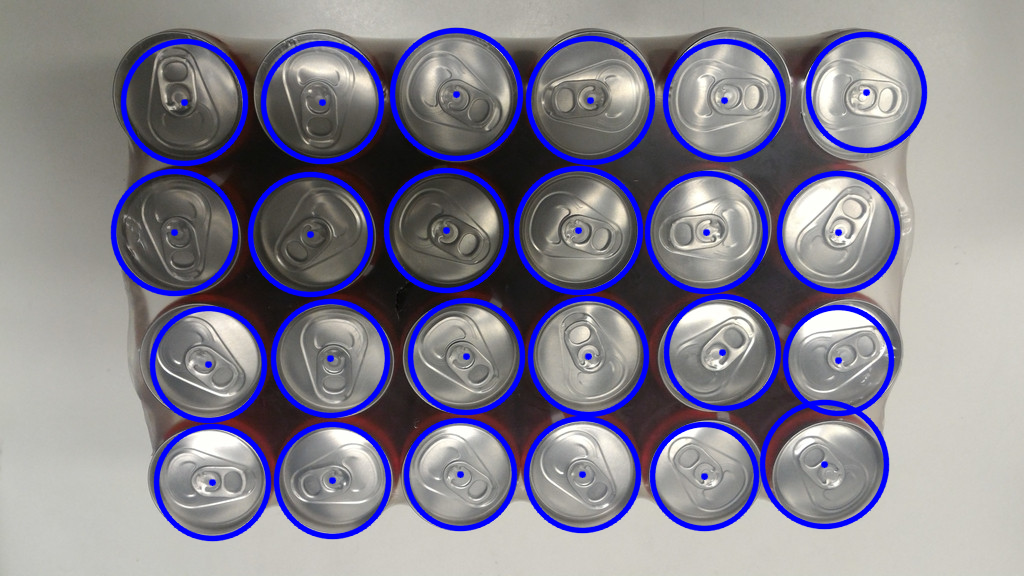
\includegraphics[width=0.9\textwidth]{../outputs/image6_canny_r5065.png}
    \caption{Результат преобразования Хафа для окружностей диапазона радиусов $[50, 65]$}
\end{figure}

\subsection{Изображение №2}

\begin{figure}[H]
    \centering
    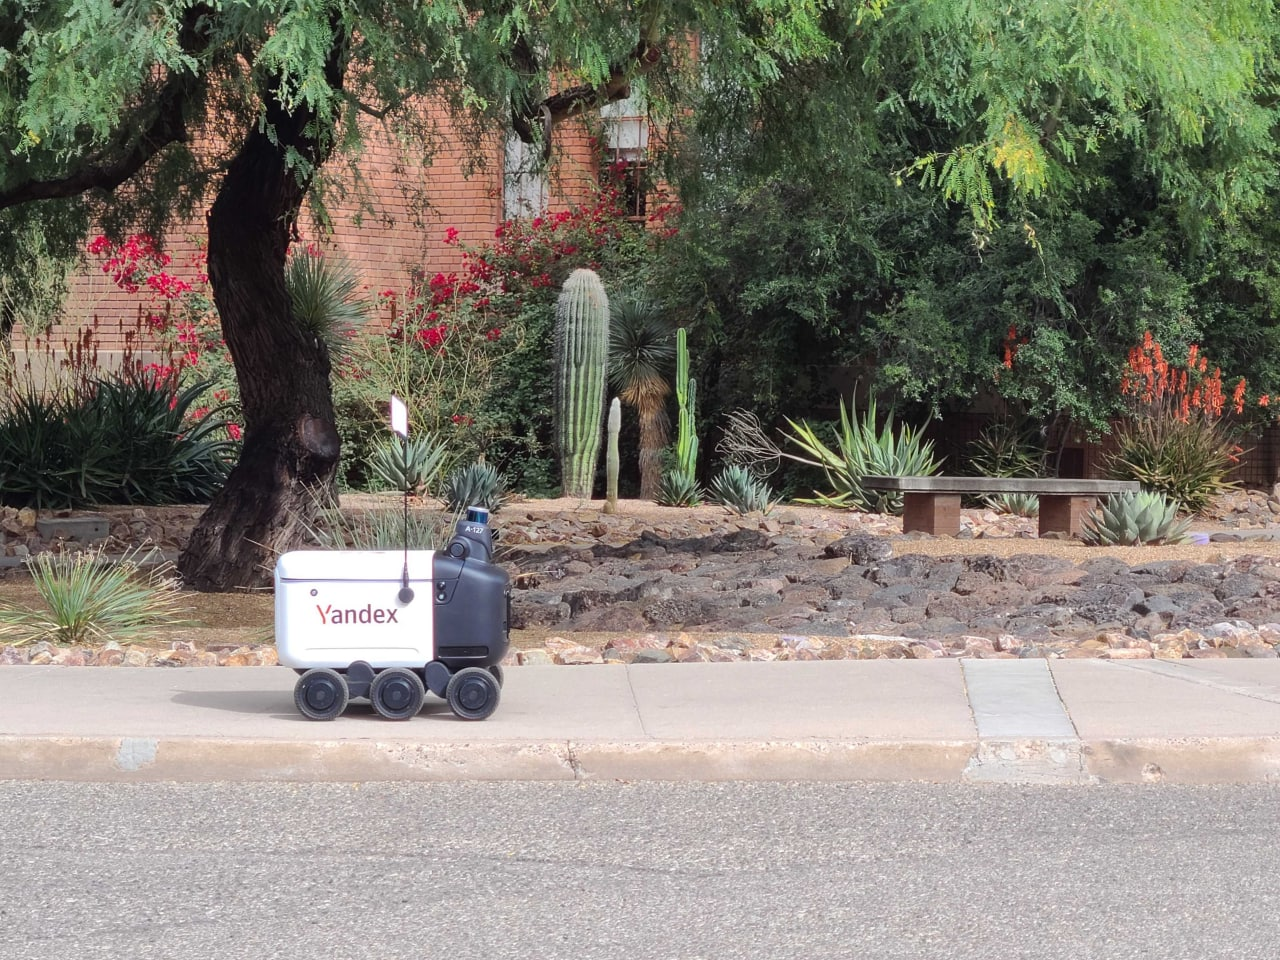
\includegraphics[width=0.9\textwidth]{../source/7.png}
    \caption{Исходное изображение}
\end{figure}

\subsubsection{Исходное изображение}

% \paragraph{Поиск окружностей определенного радиуса}

\begin{figure}[H]
    \centering
    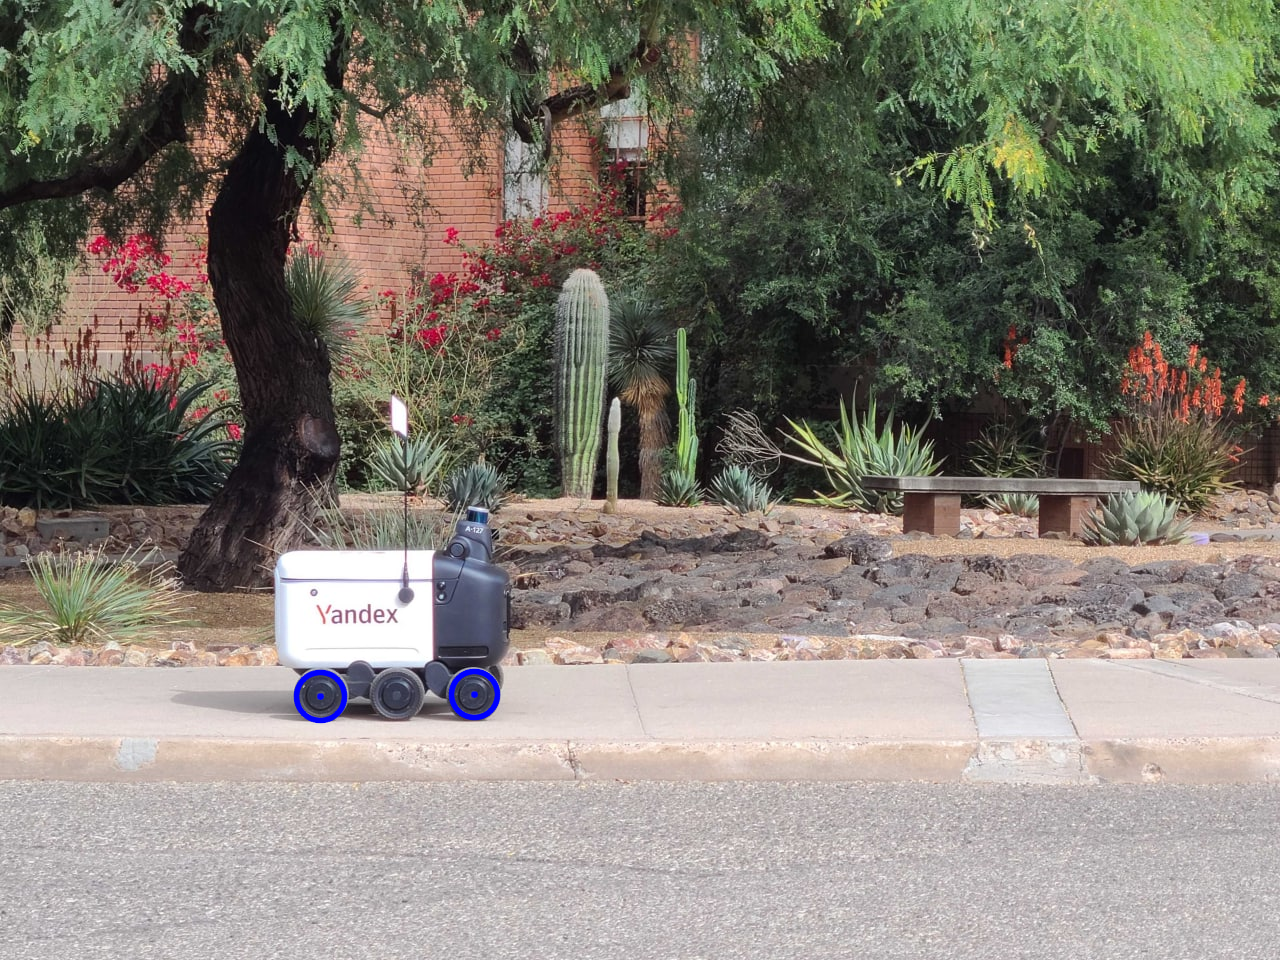
\includegraphics[width=0.9\textwidth]{../outputs/image7_ordinary_r25.png}
    \caption{Результат преобразования Хафа для окружностей радиуса 25}
\end{figure}

% \paragraph{Поиск окружностей определенного диапазона радиусов}

\begin{figure}[H]
    \centering
    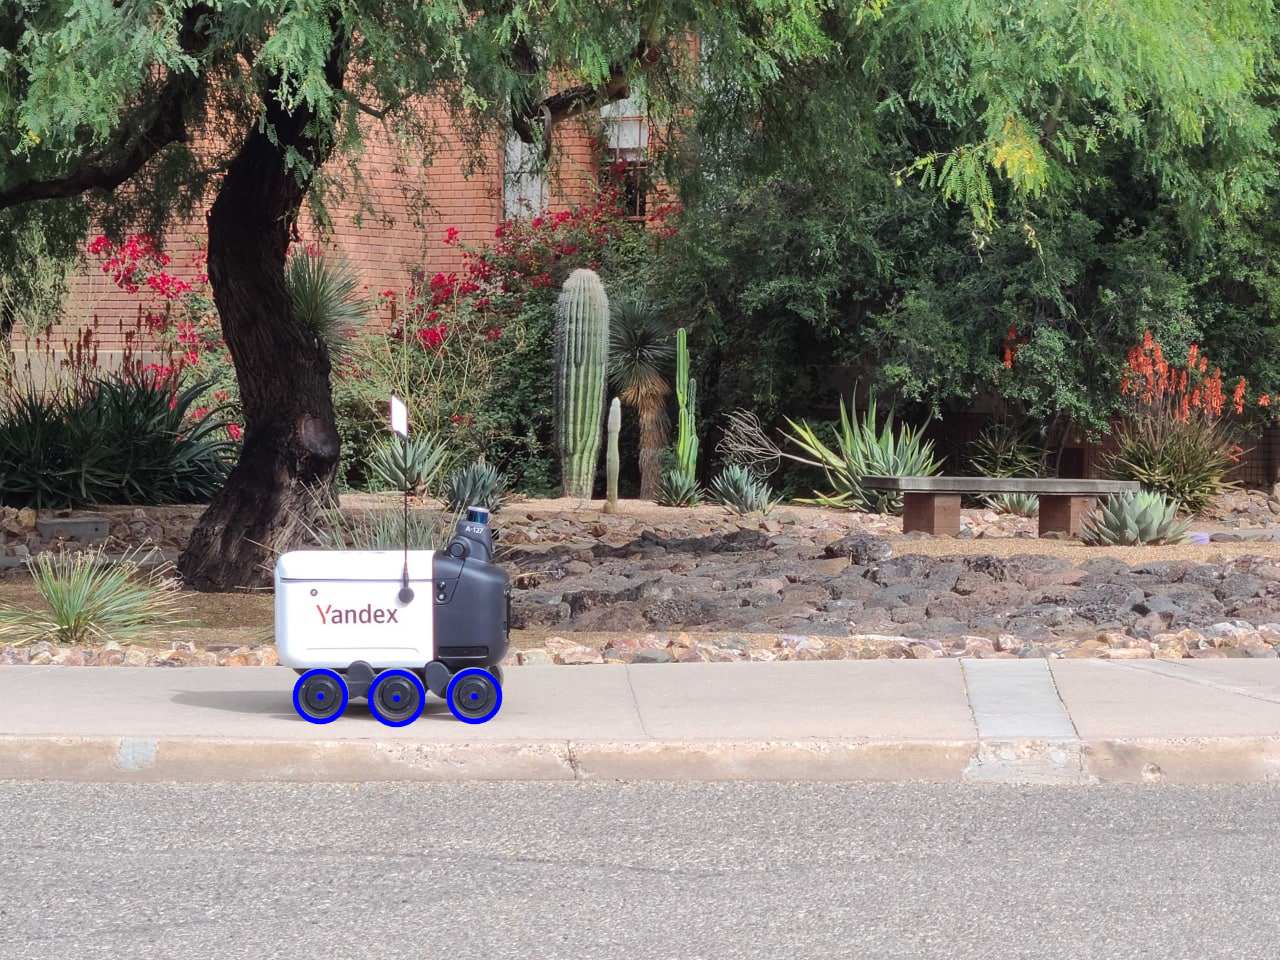
\includegraphics[width=0.9\textwidth]{../outputs/image7_ordinary_r2030.png}
    \caption{Результат преобразования Хафа для окружностей диапазона радиусов $[20, 30]$}
\end{figure}

\subsubsection{Обработанное алгоритмом Кэнни}

% \paragraph{Поиск окружностей определенного радиуса}

\begin{figure}[H]
    \centering
    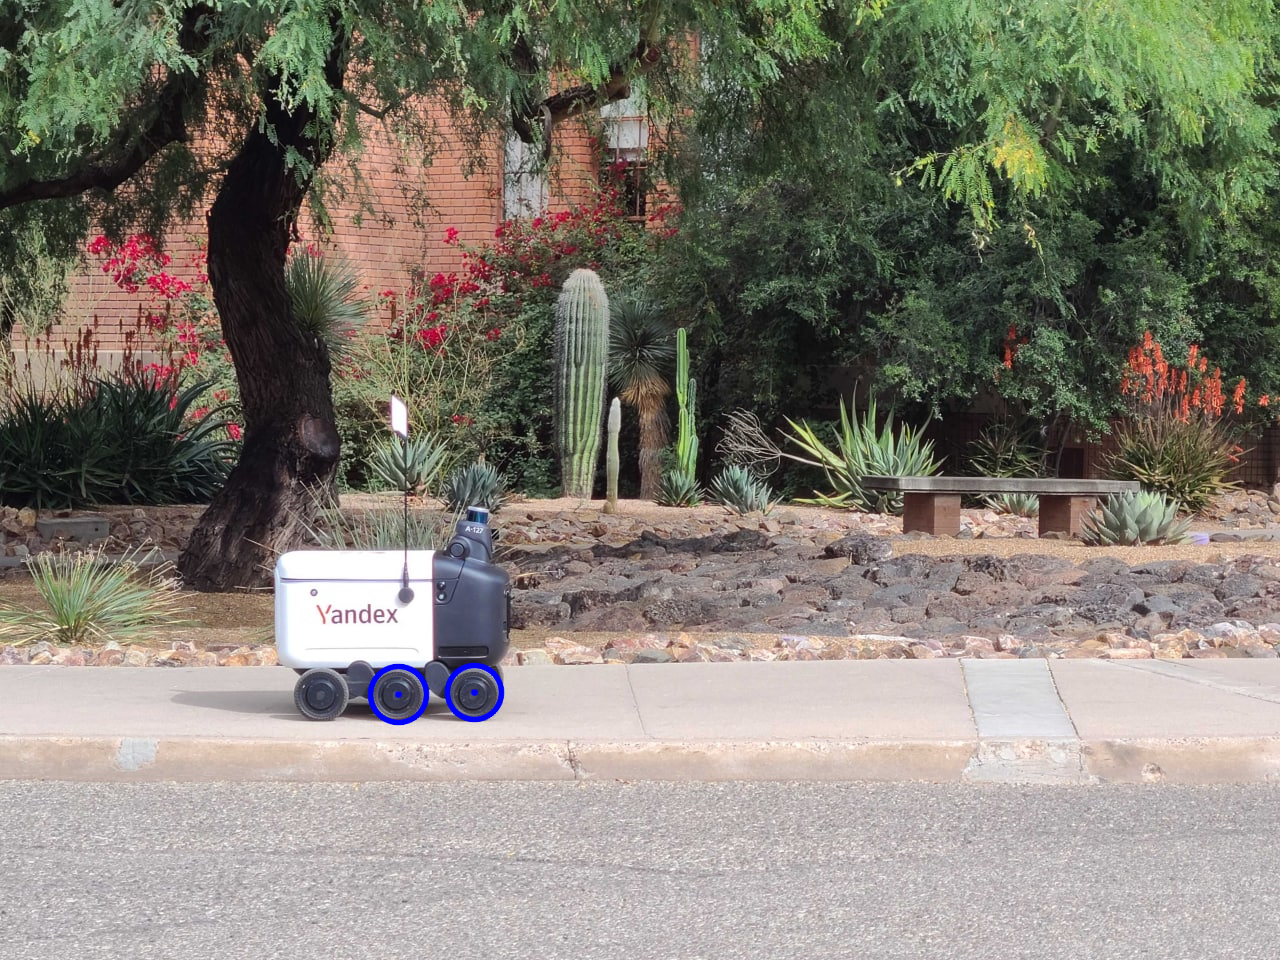
\includegraphics[width=0.9\textwidth]{../outputs/image7_canny_r35.png}
    \caption{Результат преобразования Хафа для окружностей радиуса 35}
\end{figure}

% \paragraph{Поиск окружностей определенного диапазона радиусов}

\begin{figure}[H]
    \centering
    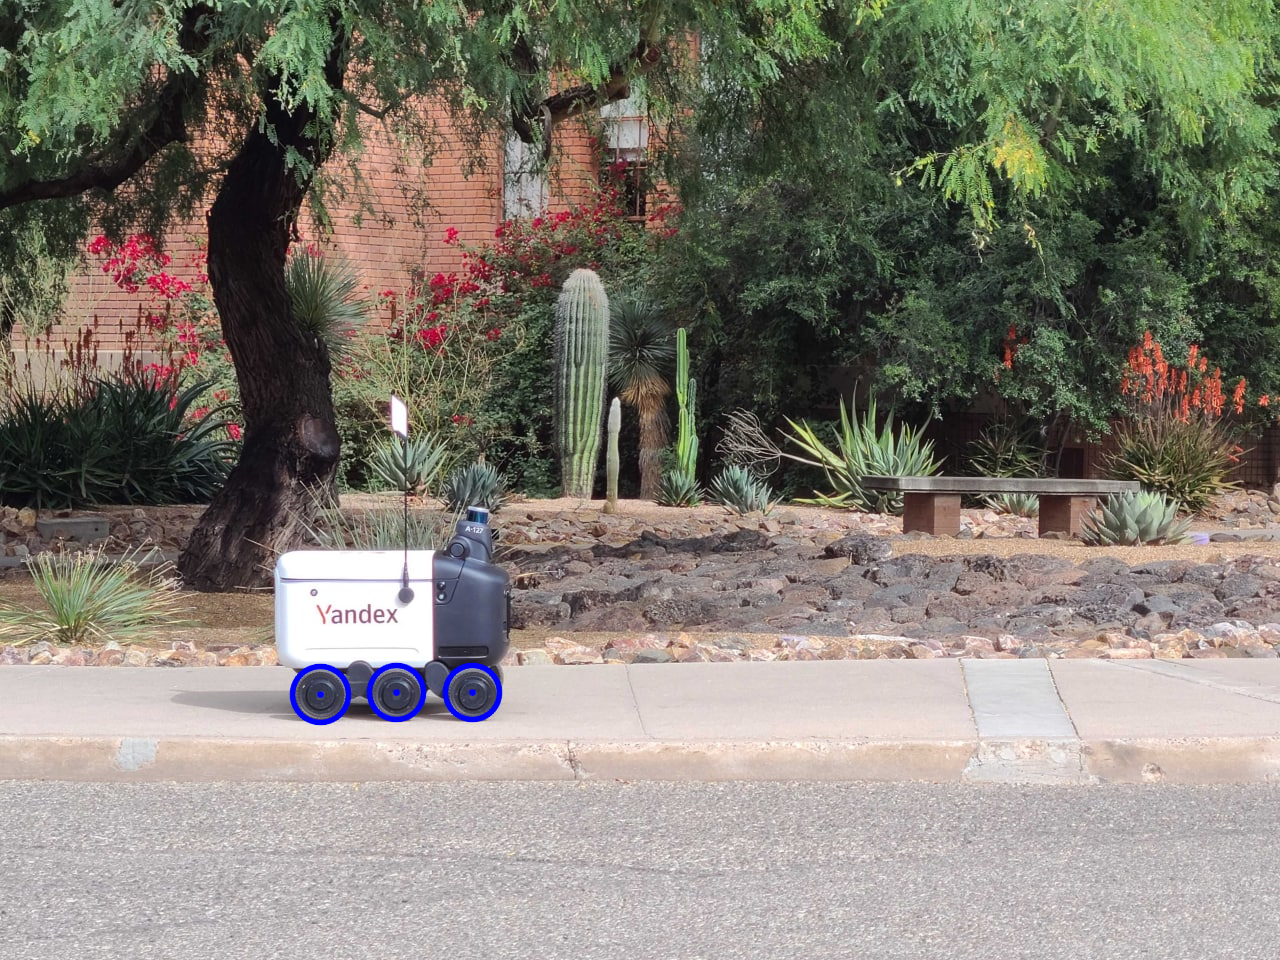
\includegraphics[width=0.9\textwidth]{../outputs/image7_canny_r3045.png}
    \caption{Результат преобразования Хафа для окружностей диапазона радиусов $[35, 45]$}
\end{figure}


\subsection{Изображение №3}

\begin{figure}[H]
    \centering
    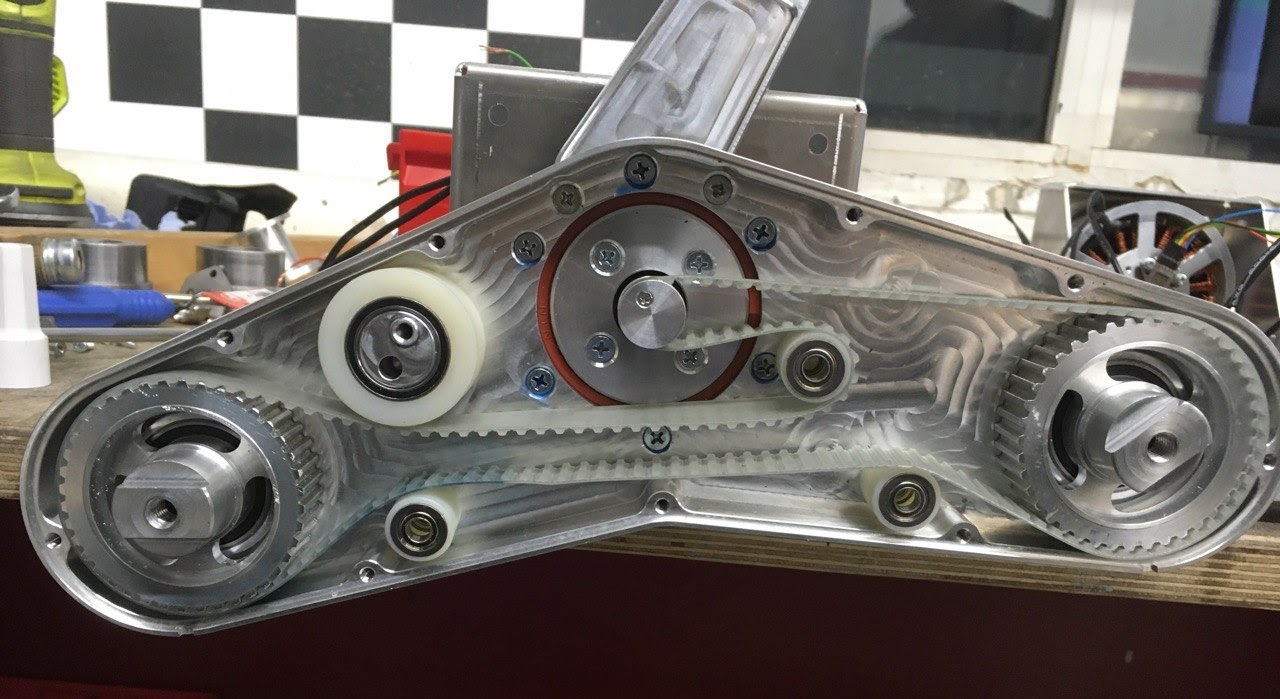
\includegraphics[width=0.9\textwidth]{../source/8.png}
    \caption{Исходное изображение}
\end{figure}

\subsubsection{Исходное изображение}

% \paragraph{Поиск окружностей определенного радиуса}

\begin{figure}[H]
    \centering
    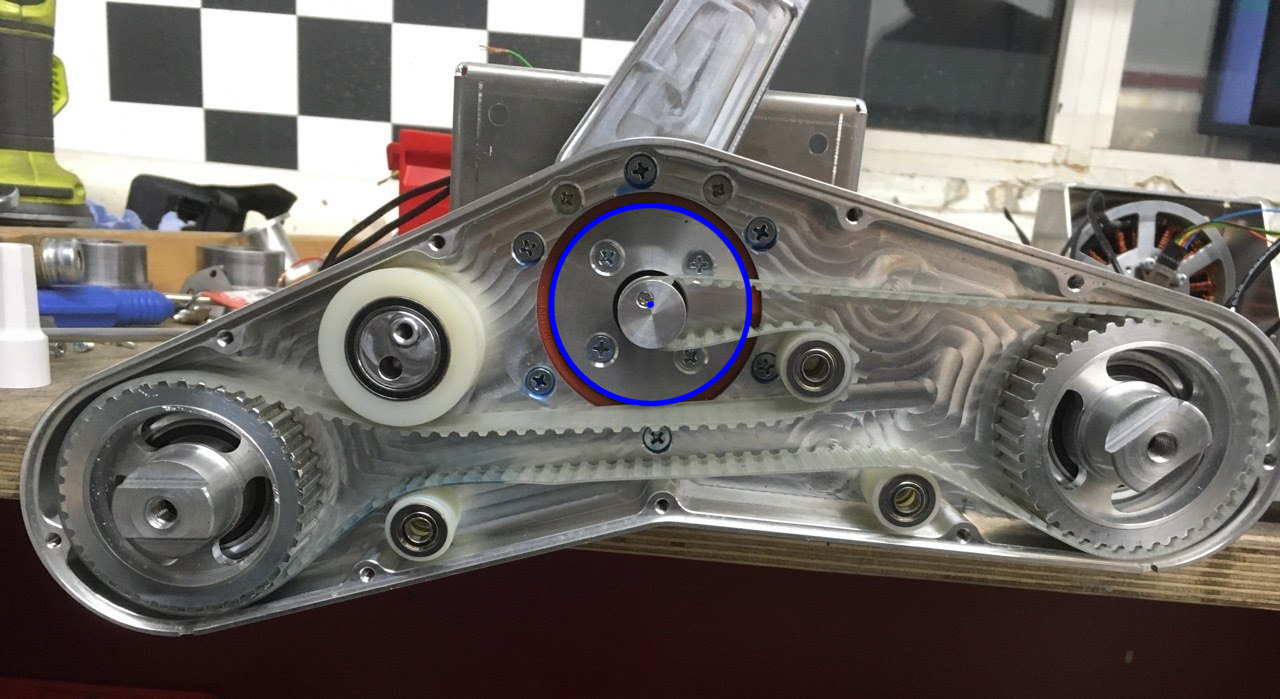
\includegraphics[width=0.9\textwidth]{../outputs/image8_ordinary_r100.png}
    \caption{Результат преобразования Хафа для окружностей радиуса 100}
\end{figure}

% \paragraph{Поиск окружностей определенного диапазона радиусов}

\begin{figure}[H]
    \centering
    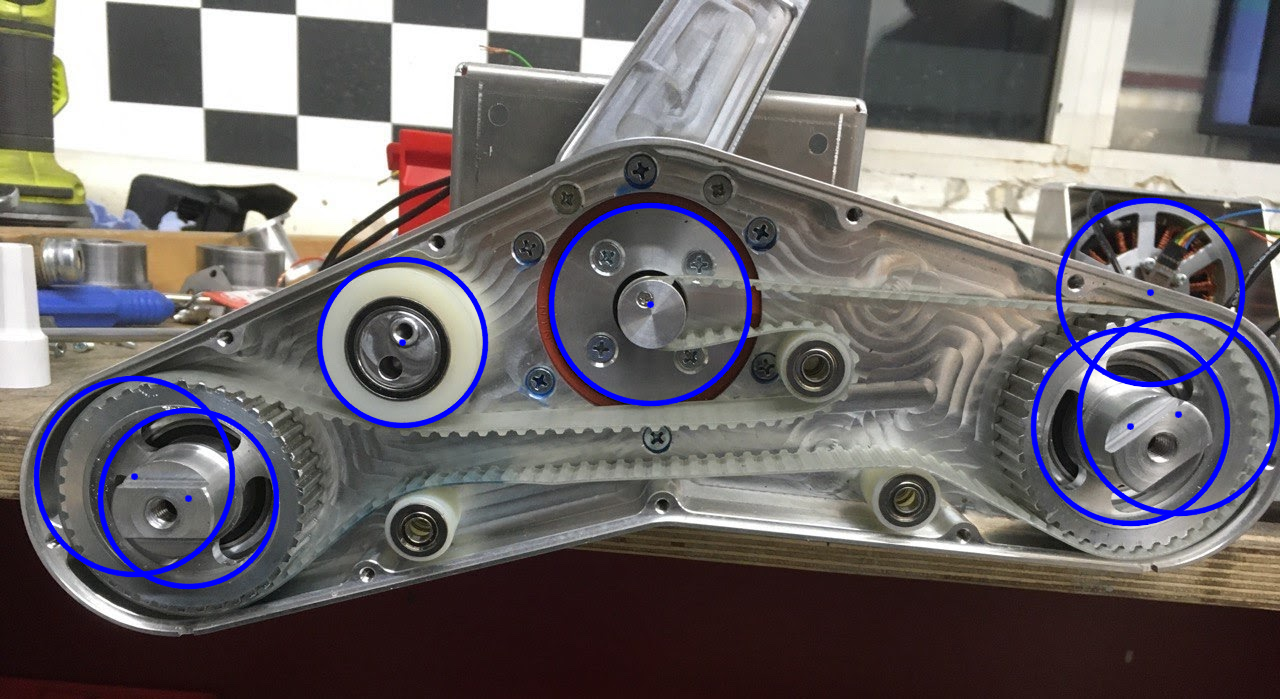
\includegraphics[width=0.9\textwidth]{../outputs/image8_ordinary_r80100.png}
    \caption{Результат преобразования Хафа для окружностей диапазона радиусов $[80, 100]$}
\end{figure}

\subsubsection{Обработанное алгоритмом Кэнни}

% \paragraph{Поиск окружностей определенного радиуса}

\begin{figure}[H]
    \centering
    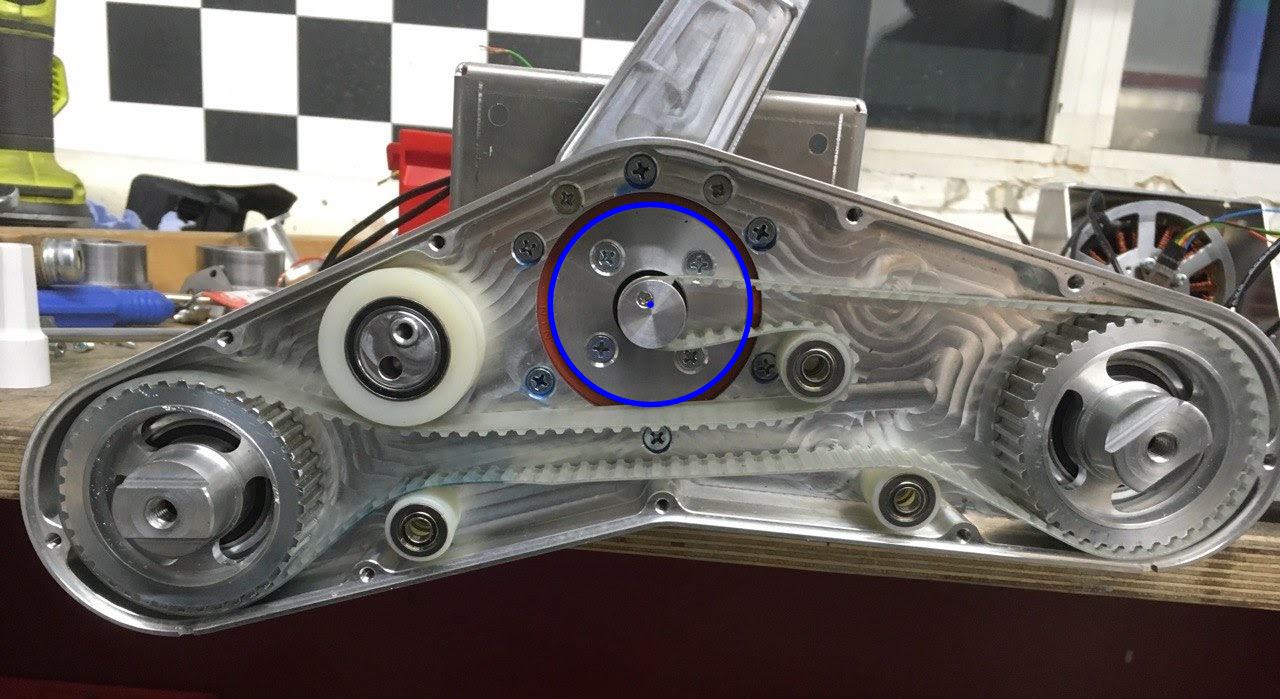
\includegraphics[width=0.9\textwidth]{../outputs/image8_canny_r100.png}
    \caption{Результат преобразования Хафа для окружностей радиуса 100}
\end{figure}

% \paragraph{Поиск окружностей определенного диапазона радиусов}

\begin{figure}[H]
    \centering
    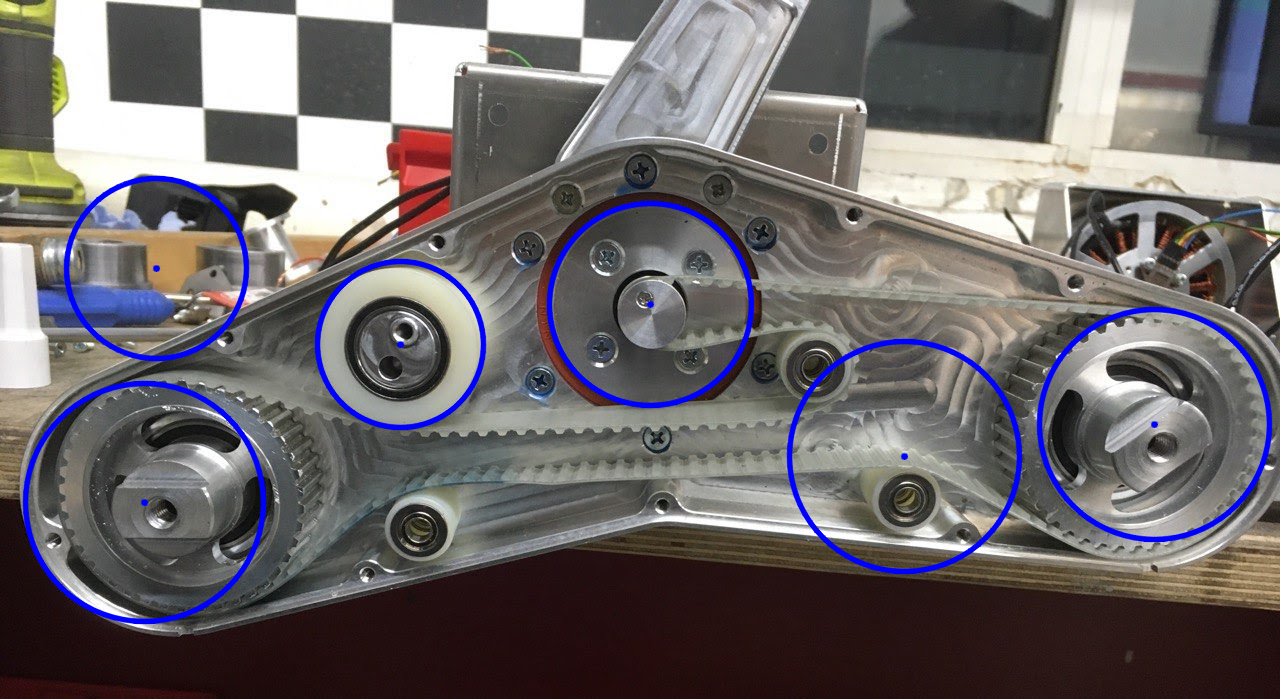
\includegraphics[width=0.9\textwidth]{../outputs/image8_canny_r80110.png}
    \caption{Результат преобразования Хафа для окружностей диапазона радиусов $[80, 100]$}
\end{figure}


\section{Ответы на вопросы}

\newcounter{question}
\setcounter{question}{0}

\newcommand{\question}[1]{\item[Q\refstepcounter{question}\thequestion.] #1}
\newcommand{\answer}[1]{\item[A\thequestion.] #1}

\begin{itemize}

\question{Какая идея лежит в основе преобразования Хафа?}
\answer{Преобразование Хафа - это метод анализа изображений, используемый для обнаружения форм геометрических объектов, особенно в компьютерном зрении и обработке изображений. Идея, лежащая в его основе, заключается в преобразовании координатных пространств, чтобы перейти от пространства параметров объектов (например, прямых или окружностей) к пространству параметров линий, сгруппировав их по общим свойствам.

В контексте обнаружения прямых на изображениях, преобразование Хафа переводит пиксели изображения в параметрическое пространство, где каждая точка представляет потенциальную прямую в исходном изображении. После этого используется аккумуляторный массив для определения областей, в которых сосредоточены прямые линии. Это позволяет выделять прямые линии, даже если они прерывисты или находятся под углом.

Идея заключается в том, чтобы перевести задачу поиска прямых на изображении в задачу поиска точек в параметрическом пространстве, что делает процесс более эффективным и менее чувствительным к шуму и другим артефактам на изображении.}

\question{Можно ли использовать преобразование Хафа для поиска
произвольных контуров, которые невозможно описать аналитически?}
\answer{

Да, преобразование Хафа можно применять не только для обнаружения прямых линий, но и для поиска произвольных контуров или форм, которые невозможно описать аналитически. Это достигается за счет того, что преобразование Хафа позволяет искать не только прямые линии, но и другие геометрические формы, такие как окружности или эллипсы, путем адаптации преобразования и выбора соответствующих параметров.

Например, для поиска произвольных контуров на изображении можно использовать преобразование Хафа с параметризацией, которая позволяет искать точки, соответствующие кривым или формам, таким как круги, эллипсы или даже неопределенные контуры. Затем можно применять дополнительные методы, такие как кластеризация или фильтрация, для идентификации и извлечения конкретных контуров или форм из набора найденных точек в преобразованном пространстве параметров.

Таким образом, преобразование Хафа является мощным инструментом для обнаружения различных геометрических форм на изображениях, включая произвольные контуры, которые могут быть сложно описать аналитически.
}

\question{Что такое рекуррентное и обобщенное преобразования Хафа?}
\answer{
    Рекуррентное и обобщенное преобразования Хафа являются расширениями классического преобразования Хафа, которые были разработаны для более эффективного обнаружения объектов на изображениях, особенно в условиях повышенного шума или сложной геометрии.
    
    Рекуррентное преобразование Хафа: Это модификация классического преобразования Хафа, которая включает процесс итеративного уточнения найденных параметров объектов путем повторного применения преобразования Хафа к изображению с последующим объединением результатов. Это позволяет повысить точность обнаружения объектов и снизить влияние шума.
    
    Обобщенное преобразование Хафа: Это расширение, которое позволяет обнаруживать объекты с произвольными формами, а не только с фиксированными, такими как прямые или окружности. В обобщенном преобразовании Хафа используются более сложные модели объектов, и соответствующие преобразования применяются к изображению для поиска параметров этих моделей. Это делает метод более гибким и способным к обнаружению более широкого спектра объектов.}


\question{Какие бывают способы параметризации в преобразовании Хафа?}
\answer{
    Преобразование Хафа позволяет обнаруживать объекты на изображении, представляя их в параметрическом пространстве. Способы параметризации в преобразовании Хафа зависят от типа объекта, который вы хотите обнаружить. Некоторые из основных способов параметризации включают:

Для прямых линий:

Параметризация в полярных координатах:

Параметризация в декартовых координатах: Используются параметры, такие как полуоси 

Для окружностей:

Параметризация в полярных координатах: $r$ - радиус и координаты центра

Для эллипсов:

Параметризация в декартовых координатах: Используются параметры, такие как полуоси и координаты центра и угол поворота.

В случае обобщенного преобразования Хафа или адаптации для обнаружения произвольных форм, параметры могут варьироваться в зависимости от конкретной геометрической модели, используемой для представления объекта.
Выбор определенного способа параметризации зависит от характеристик объекта и задачи обнаружения, а также может влиять на эффективность и точность процесса обнаружения.}

\end{itemize}

 % Content

\end{document}